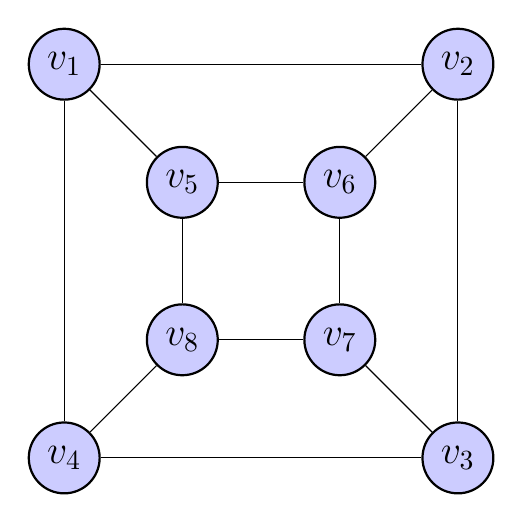
\begin{tikzpicture}[
  scale=1,
  vnode/.style={circle, fill=blue!20, draw=black, thick, minimum size=9mm, inner sep=0pt, font=\Large}
]
  % Vértices del cuadrado exterior
  \node[vnode] (v1) at (0.0, 5.0) {$v_1$};
  \node[vnode] (v2) at (5.0, 5.0) {$v_2$};
  \node[vnode] (v3) at (5.0, 0.0) {$v_3$};
  \node[vnode] (v4) at (0.0, 0.0) {$v_4$};

  % Vértices del cuadrado interior
  \node[vnode] (v5) at (1.5, 3.5) {$v_5$};
  \node[vnode] (v6) at (3.5, 3.5) {$v_6$};
  \node[vnode] (v7) at (3.5, 1.5) {$v_7$};
  \node[vnode] (v8) at (1.5, 1.5) {$v_8$};

  % Aristas
  \foreach \from/\to in {v1/v2, v2/v3, v3/v4, v4/v1,
                         v5/v6, v6/v7, v7/v8, v8/v5,
                         v1/v5, v2/v6, v3/v7, v4/v8}
    \draw (\from) -- (\to);
\end{tikzpicture}
